% Chapter Template

\chapter{Python Reshape}
\label{Python Reshape}

\section{Python program}

%----------------------------------------------------------------------------------------
%	SUBSECTION 1
%----------------------------------------------------------------------------------------

\subsection{Initialization and input values}

The Python code developed is inspired from a previous one, done in MatLab by \parencite{Reference14} for DCB tests. MMCG specimen was created from DCB one, so it was logical to use this program with an adaptation to Python tools. 

The main purpose of this tool is to compute all the information given by DIC and obtain the energy release rate. To do that, it was remind in \ref{eq:Energy release rate equation} that many parameters must be input. Some of them are constant and was measured before or after the test. It is the case for $a_{0}$ and "b" parameters, respectively the initial crack length and the thickness of the specimen analysed. It is dfined in four big parts.

So a first program, allowing to combine all the constants by creating a structure as the one below, was done. It is called database and the following one is the example from the third Okoume specimen of the first experiment database:
\lstinputlisting[language=Python, firstline=1, lastline=9]{Codes/Database.py}

\begin{lstlisting}[language=Python]
	LX, H = 29.3, 1624  # mm / pixel
	if Job == 'e1o3':
	##########################################################################
	# pixel to mm magnification factor
	Test.mm2pixel = LX / H
	# Load conversion factor - testing machine
	Test.LoadConvFactor = 1000  # from kN to N
	# Displacement conversion factor - testing machine
	Test.DisplConvFactor = 2.0  # mm/V (gain = 20 mm)
	Test.thickness = 14 # unit  mm
	Test.a0 = 24.5 # unit  mm
\end{lstlisting}


\lstinputlisting[language=Python, firstline=11, lastline=19]{Codes/Database.py}

Thanks to this database file, open in the main code file, many calls can be done and allow to synthesize the main code. Of course one database was created for each specimen andinput in a single folder, due to the difference between values as the precrack length or the thickness of the specimen. Other values as the "Test.LoadConvFactor" will always be the same. Indeed, in this work, the load values, given by MTS press \ref{fig:Fig8} are given in \si{\kilo\newton}, so a coefficient of 1000 must be added to obtain coherants results.

All the values from MatchID must be read and the displacement or load from the Hydraulic Press have to been stored in Python variables. 

\begin{lstlisting}[language=Python]
# determining the number of stages by inspecting MatchID processing files
stages = glob.glob(os.path.join(cwd, 'DCB_002_*.tif.dat'))
MatchID.stages = stages.__len__()
print('Number of stages: ', str(MatchID.stages))
\end{lstlisting}

The first step is to store in a parameter, the number of stages by looking to the number of images captured by MatchID. As it is visible, variables are created, in a structure named MatchID. Here, the number of stages is stored in MatchID.stages variable. This MatchID structure is present in the database, because it is linked to each specimen. Indeed, the number of images changes from one test to another. So another part of the database is linked to MatchID settings and add information linked to this structure:  

\begin{lstlisting}[language=Python]
	# Summary of DIC Settings
MatchID.CorrelationCoef = 'ZNSSD'
MatchID.InterpolationOrder = 'Bicubic spline'
MatchID.TransformationOrder = 'Affine'
MatchID.Subset, MatchID.Step = 15, 13
# Summary of Strain Settings
MatchID.StrainWindow = 5
MatchID.StrainConvention = 'GreenLagrange'
MatchID.StrainInterpolation = 'Q4'
# Area of Interest
MatchID.Roi_PolyXi, MatchID.Roi_PolyYi = 52, 259
MatchID.Roi_PolyXf, MatchID.Roi_PolyYf = 1587, 1119
\end{customFrame}

It is possible to use thanks to this part, the type of subset used, the steps, the strain window and intrpolation, previously chosen looking on the best parameters on MatchID curves. Then, the displacements and load of every stages must be stored to. In order to do it, an iterative loop is created :

\begin{lstlisting}[language=Python]
# U displacement
UX = np.zeros((MatchID.SubsetsY, MatchID.SubsetsX, MatchID.stages))
tic()
for i in np.arange(0, MatchID.stages, 1):
readstr = #Name of the test
print('reading : ',readstr)
pathdados = os.path.join(cwd,'u',readstr)
aux = np.genfromtxt(pathdados, skip_header=0, delimiter=';')
UX[:, :, i] = aux[:, :-1]*Test.mm2pixel # unit: mm
print(f'{toc():.1f} seg')
\end{lstlisting}

This loop stores the displacement on U direction, but an other similar one do the same on V direction. Ux is a Matrix filled by the reading of MatchID.subset file and the number of stages. Then it is multiply by the convector factor from \si{\pixel} to \si{\milli\meter}. 

%----------------------------------------------------------------------------------------
%	SUBSECTION 3
%----------------------------------------------------------------------------------------

\subsection{Determination of the CTOD} 

After computing all the datas from the database, a second part is computed. It is linked to the Crack Tip Opening Displacement (CTOD). Indeed, this factor has impact on the cohesive law. MatchID is a great tool which does some work for the user. That is why, some of the information from the software program were put in the Database, as in the next code with the ZOI dimensions: 
\begin{lstlisting}[language=Python]
# Allied Manta G-505B
H, V  = 2448, 2050 # unit: pixels
# 'TC2336' telecentric lens
LX, LY = 34.98, 29.18 # unit: mm
\end{lstlisting}

Then, two matrix are created. There are first, declared and made of zeros :

\begin{lstlisting}[language=Python]
CTODI  = np.zeros((ud_lim, 3, MatchID.stages))
# Vup, Vdown, ||Vup-Vdown||
CTODII = np.zeros((ud_lim, 3, MatchID.stages))
\end{lstlisting}

As shown in the code, the dimensions of the matrix take in account the number of stages, so the number of images. Indeed, the interest of the CTOD is to be folowed at each stage. 

Then, a loop is created, allowing to put information into others vectors

\begin{lstlisting}[language=Python]
for J in np.arange(0, MatchID.stages, 1):
# mode I:
uYtemp = np.copy(UY[:, :, J])
CTODI[:, 0, J] = np.flipud(uYtemp[a0.Y - ud_lim: a0.Y, a0.X])
CTODI[:, 1, J] = uYtemp[a0.Y: a0.Y + ud_lim, a0.X]
CTODI[:, 2, J] = np.abs(CTODI[:, 1, J] - CTODI[:, 0, J])
\end{lstlisting}

An other one is also created to compared to mode II values. In the current case, the mode II can be approximate around zero, because it is a mode I test. Then all the values are obtained, for each COD pair until ud$_$lim which is in this case equal to 10. By looking to this different curves, the chosen COD pair is chosen and a curve is plot looking to the values for this parameter chosen by the user. 

\begin{figure}[h]
	\centering
	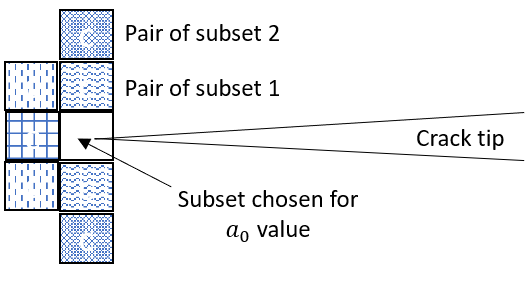
\includegraphics[scale=0.7]{Figures/Subset_choice}
	\decoRule
	\caption[Subset choice and pair of subset around]{Pair of subset around the $a_{0}$ subest chosen}
	\label{fig:subest_chosen}
\end{figure}

Finally, the way to obtain CTOD, alos need a well $a_{0}$ choice. Indeed, the chosen subset as presented on \ref{fig:subest_chosen}, will be determinant. Considering the image as a matrix composed of subset, the chosen subset as a position given by his m row and n column. To determinate the opening, it is necessary to have a look on the subsets in the same n column but at a different line. Indeed, the chosen subset will be the first one affected by the crack, that means, that information on the subset will not have importance anymore. While, looking to subset up and down allow to follow the displacement of the crack tip and measure it. The fact is to determine which pair of subsets is the best. The ones at the row n-1 and n+1, but maybe these ones will be on the crack at a given stage and will lose all the necessary information. That is why, an important choice must be done. Here COD pair was fixed equal to two. So the subset displacement analysed is the one of the pair of subset 2 on \ref{fig:subest_chosen}. Finally, by looking to these displacements, it is possible to obtain the value of the crack opening at each stages.

%----------------------------------------------------------------------------------------
%	SUBSECTION 4
%----------------------------------------------------------------------------------------

\subsection{Crack length analysis}

The third part of the code has the purpose to determine a(t), so the crack length evolution. This evolution can be compared to the time or the hydraulic press dispacement and also the load applied on the specimen. The first step is again to define everything. The displacement are stored again, the Zone Of Interest (ZOI) is defined by supressing the value out of this ZOI.
This a(t) parameter is the most difficult to obtain, indeed tools as MatchID cannot help the user to obtain the result stage by stage. The value of a(t) will be equal to $a_{0}$ fixed by the user and add to a $\Delta a$ which is the value of the crack length, evolving in time due to the applied force.

\begin{lstlisting}[language=Python]
displ_x = UX[:,:,J]
displ_y = UY[:,:,J]
# resize RoI containing the crack growth process
if roi == 'crop':
displ_x = displ_x[Y_i:Y_f,X_i:X_f]
displ_y = displ_y[Y_i:Y_f,X_i:X_f]

# find the dimensions of the matrix
m = displ_x.shape[0] #  y - row
n = displ_x.shape[1] # x - column
# find the matrix with the displacements
displ = (displ_x**2 + displ_y**2)**0.5
# preallocation: zeros
n_zeros = np.zeros((m, 1))
m_zeros = np.zeros((1, n+1))
\end{lstlisting}

After defining all the parameters, the displacement of the crack tip is observed thanks to some calculus on the subsets. 

\begin{lstlisting}[language=Python]
displ_A = np.vstack((np.hstack((displ,n_zeros)), m_zeros))/4
# divided by 4 because sum: displ_A+displ_B+displ_C+displ_D
displ_B = np.vstack((np.hstack((n_zeros,displ)), m_zeros))/4
displ_C = np.vstack((m_zeros, (np.hstack((displ, n_zeros)))))/4
displ_D = np.vstack((m_zeros, (np.hstack((n_zeros, displ)))))/4
# auxiliar matrix 2 edges; 4 within the matrix 'matr_transf'
matr_transf = np.ones((m+1, n+1))
matr_transf[:, 0] = 2
matr_transf[:, -1] = 2
matr_transf[0, :] = 2
matr_transf[-1, :] = 2
matr_transf[0, 0] = 4
matr_transf[0, -1] = 4
matr_transf[-1, 0] = 4
matr_transf[-1, -1] = 4
grid_values = (displ_A + displ_B + displ_C + displ_D)*matr_transf
# displacements of each corner on the facet
displ_A = grid_values[0:-1, 0:-1]
displ_B = grid_values[0:-1, 1:]
displ_C = grid_values[1:, 0:-1]
displ_D = grid_values[1:, 1:]
# oblique distance between facet centroids
displ_CA = np.abs(displ_C-displ_A)
displ_DB = np.abs(displ_D-displ_B)
# auxiliar function for the crack tip location criterion
K = np.maximum(displ_CA, displ_DB)
avgK = np.nanmean(K) #mean ignoring nan values.
stdK = np.nanstd(K)
maxK = np.nanmax(K)
if maxK < avgK + inb*stdK:
J = J + 1
else:
JJ = 0
\end{lstlisting}

Here, all the matrix, composed of the subsets from the Zone of Interest are changed by the different steps shown overhead. All the subsets are considered four by four and operatins are done on them. The displacement from one compared to it neighbor are computed. Then average and maximum values are obtained for each subsets of the ZOI and put into K matrix. By using the $a_{0}$ data and looking to the alpha parameter, permitting to compute the best shape of a(t), having the more precise values but numerous ones also, a(t) is obtained with a similar methode. It must be noticed, that to determinate a(t) parameter, $\alpha$ parameter is needed. This one is used on matrix as the M matrix. Indeed, M matrix represents, for a given stage, the crack length by having bigger value in the crack area as shown on \ref{fig:Fig11} : 

\begin{figure}[h]
	\centering
	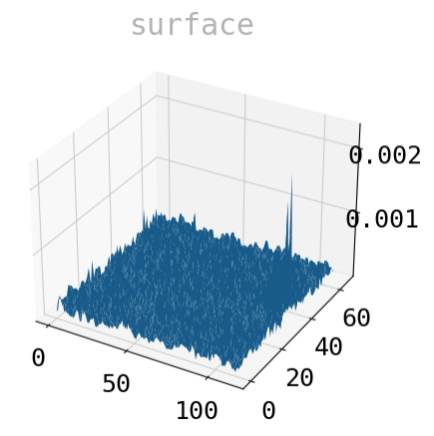
\includegraphics[scale=0.5]{Figures/M_matrix}
	\decoRule
	\caption[M matrix]{M matrix, obtained by running python code}
	\label{fig:Fig11}
\end{figure}

As it is visible, if the user is looking too close, the noise of the values will avoid a good analyze, but by looking too high on the matrix, the crack length value will not be accurate. To move and have a precise idea of the way the user can watch the M matrix, it is important to use $\alpha$. Alpha parameter is like a cutting tool which allows to be as close as the noise without troubles.
To approximate the $\alpha$ value, a correlation factor is searched by least square regression method. The objective it to have the best linear part. A plot is created to show which stage is the most appropriate as on \ref{fig:Fig12}.

\begin{lstlisting}[language=Python]
	### 2 criterion for checking stage
	####
	inb = 3
	# standard deviation * inb (to be checked by user)
	# inb = 1: 68.3 %
	# inb = 2: 95.4 %
	# inb = 3: 99.7 %
\end{lstlisting}

It is possible to adapt the alpha parameter precision by choosing a different "inb" as presented in the code overhead. Indeed, the correlation factor change depending on this criterion. The chosen stage is the one, before the beginning of the crack propagation, but the nearest to the expansion of a(t) length.

\begin{figure}[h]
	\centering
	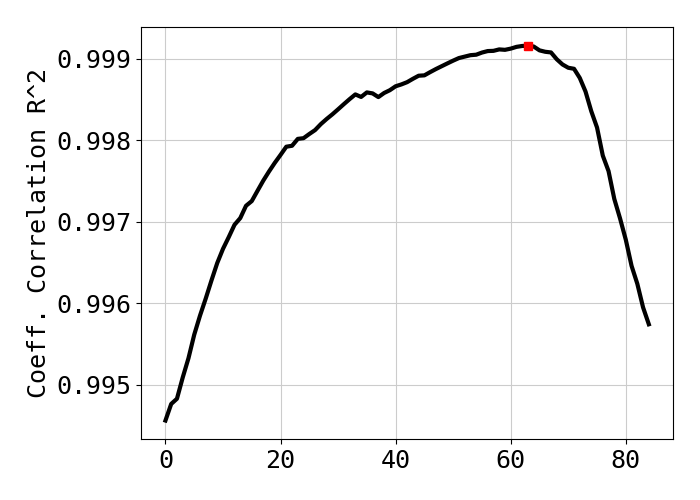
\includegraphics[scale=0.3]{Figures/Correlation_factor}
	\decoRule
	\caption[R correlation factor]{R correlation factor allowing to know which load and disalcement is linked to crack beggining.}
	\label{fig:Fig12}
\end{figure}

This method was the one used by \parencite{Reference14} on MatLab, and have already prooved a good functionnement.

%%----------------------------------------------------------------------------------------
%%	SUBSECTION 5
%%----------------------------------------------------------------------------------------
\subsection{Compliance and Energy values}

The last part of the code consists in using all the calculated parameters, in order to obtain the energy release rate. It is done by computin the G formula as presented below.

\begin{equation}
	G_{c}= \frac{F_{c}^2}{2b} (\frac{\Delta C}{\Delta a})_{d} 	
	\label{eq:Energy release rate equation}
\end{equation}

This equation already given, is written on Python as :

\begin{lstlisting}[language=Python]
a_t = crackL_J_mm[:,chos_alp]

C = MatchID.displ/MatchID.load

# P**2/2/B* dC / da
ALP = (MatchID.load**2)/(2*Test.thickness)

# C = MatchID.displ/MatchID.load

# BET = C/a_t #changing the value of alpha from the crack length will change G values
#
G = ALP*BET
# G = np.dot(ALP,BET)
\end{lstlisting}

In this case, the formula used, is the simplest one, which allow to easily obtain C by dividing the displacement from hydraulic press by the load. These values are stored in MatchID variable, allowing to synthesize all the datas in one per image (stage). An average are done on the seven values between two images. This fact can also involve a little mistake.
Therefore, as explained in "alpha" and "a(t) determination" sections, the crack length depends on alpha parameter. So some curves are ploted depending on "a(t)" matrix changes according to the alpha. The best R-curves must be determined for the most precise crack length. So it is necessary to find a great alpha parameter to have these final values without huge mistake.

\begin{lstlisting}[language=Python]
# write array results on a csv file:
RES = np.array([MatchID.displ[:], MatchID.load[:], C[:], COD.wI[:], a_t[:], G[:]])
RES = np.transpose(RES)
\end{lstlisting}

At least, values as the displacement, the load, the compliance, the CTOD, the crack length and the energy release rate, are stored into a matrix and then exported to .csv files. It allows to save datas, but also to compute everytthing in Excel in addition to python processing tool.

Many improvements are made on the Python code, even after this work ended. Indeed, it apears that the crack length can be better compute, in order to avoid some strange shapes of R-curves. But using the same tool for all specimens computation, even if mistakes exist, it is possible to compare datas.

%%%%%%%%%%%%%%%%%%%%%%%%%%%%%%%%%%%%%%%%%%%%%%%%%%%%%%%%%%%%%
%%%%%%%%%%%%%%%%%%%%%%%%%%%%%%%%%%%%%%%%%%%%%%%%%%%%%%%%%%%%%
%%%%%%%%%%%%%%%%%%%%%%%%%%%%%%%%%%%%%%%%%%%%%%%%%%%%%%%%%%%%%

%
%\subsection{Alpha parameter}
%
%To begin with, it is important   to determinate a parameter, that we had called $\alpha$. This one is used on matrix as the M matrix. Indeed, M matrix represents, for a given stage, the crack length by having bigger value in the crack area as shown on \ref{fig:Fig11} :
%
%\begin{figure}[h]
%	\centering
%	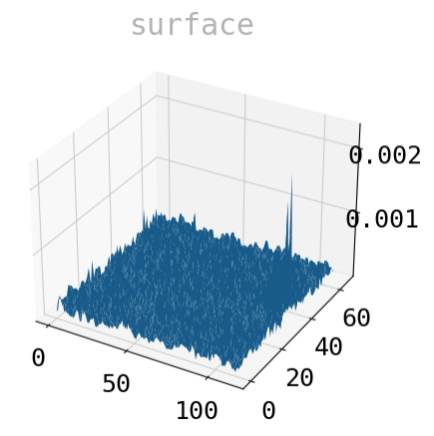
\includegraphics[scale=0.5]{Figures/M_matrix}
%	\decoRule
%	\caption[M matrix]{M matrix, obtained by running python code}
%	\label{fig:Fig11}
%\end{figure}
%As it is visible, if the user is looking too close, the noise of the values will avoid a good analyze, but by looking too high on the matrix, the crack length value will not be accurate. To move and have a precise idea of the way the user can watch the M matrix, it is important to use $\alpha$. Alpha parameter is like a cutting tool which allow to be as close as the noise without troubles.
%To approximate the $\alpha$ value, a correlation factor is searched by least square regression method. The objective it to have the best linear part.
%\begin{customFrame}
%	#### alpha evaluation
%	### Selecting stage for investigating alpha
%	####
%	# least-squares linear regression
%	porder = 1
%	xx = Test.disp # displacement (mm)
%	yy = Test.load # load (N)
%	# Data point in the linear least-squares regression
%	limsup = int(0.75*np.argwhere(max(yy)==yy)[-1])
%	# number of maximum data points for LSR
%	liminf = int(np.round((1/3)*limsup))# number of minimum data points for LSR
%	
%	xx, yy = xx[0:limsup], yy[0:limsup]
%	Rtot = np.zeros((limsup-liminf,1))
%	C_M = np.zeros((limsup-liminf,1))
%	for j in np.arange(0,limsup-liminf,1):
%	limt_sup = liminf + j
%	xfit, yfit = xx[0:limt_sup], yy[0:limt_sup]
%	p  = np.polyfit(xfit, yfit, porder)
%	C_M[j] = 1/p[0]
%	dev = yfit - np.mean(yfit) # deviations - measure of spread
%	SST = np.sum(dev**2) # total variation to be accounted for
%	resid = yfit - np.polyval(p, xfit) # residuals - measure of mismatch
%	SSE = np.sum(resid**2) # variation NOT accounted for
%	Rtot[j] = 1 - SSE/SST #  variation NOT accounted for
%	
%	# position for the best fitting point parameters
%	jmax = np.max(np.argwhere(np.max(Rtot)==Rtot))
%	J = int(liminf + jmax)
%	
%	### 2 criterion for checking stage
%	####
%	inb = 3
%	# standard deviation * inb (to be checked by user)
%	# inb = 1: 68.3 %
%	# inb = 2: 95.4 %
%	# inb = 3: 99.7 %
%	JJ = 1
%	while JJ == 1:
%\end{customFrame}
%
%\begin{figure}[h]
%	\centering
%	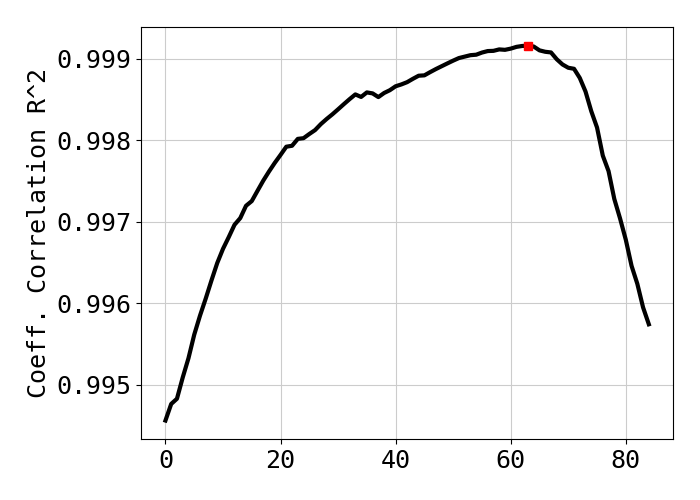
\includegraphics[scale=0.3]{Figures/Correlation_factor}
%	\decoRule
%	\caption[R correlation factor]{R correlation factor allowing to know which load and disalcement is linked to crack beggining.}
%	\label{fig:Fig12}
%\end{figure}
%
%The red dot shown on \ref{fig:Fig12}, is linked to another plot,
%
%Then a matrix representing the subsets in the Area of Interest will be created. First this matrix is composed of zero. Then, the four corners of the matrix will be used to proceed several operations on the matrix. The external lines and columns will take a value of 2 and the corners a value of 4. The distance between opposite corners is calculated and their displacements are compared. Calling K, the maximal displacement of the two corners, average K and maximum one between all the steps are compared. Again, every subset is treated and are still zero when the material is undamaged. It becomes -1 in a region where the material is damaged, and no information are treatables. And it becomes 1 where a discontinuity appears but the wood is not completely damaged like the crack tip. So, by following the farthest 1 value in the matrix, it is possible to know the last subset where the crack tip is localized. Thanks to this distance, some conversions are necessary, from subset to pixel first, and then from pixel to millimeters. Finally, the crack length is determined depending on stages so it could be linked to load or displacement, and thanks to the previous work, to CTOD. The compliance is calculated by dividing the displacement by the load. G is the last variable calculated, with all the previous variables determined, as CTOD presented below and a(t). The last plot is the R-curve representing the Energy release and the crack length.
%%----------------------------------------------------------------------------------------
%%	SUBSECTION 3
%%----------------------------------------------------------------------------------------
%
%\subsection{Determination of the CTOD}
%
%Another partof the code has the purpose to calculate the Crack Tip Opening Displacement (CTOD). MatchID is a great tool which does some work for the user. That is why, by using “wI aramis2D.csv” CTOD is almost find, depending on the time and the load applied. It is important to understand how it works.
%
%First, a part of the work is to define the zone of interest (ZOI), the one where the crack must develop. It is done on MatchID, but also on Python by using the number of the subset defined by Match ID. Then, when a subset is out of this region, it will be considered as equal to zero. Then, the subsets which are placed into the crack, or somewhere where there is a default or missing information as into the crack, the substep will be defined with a value equale to -1. Then, for all the substep around the crack, which have a real interest in the study, they will take the value equal to 1. By using this matrix of substep, now, composed of -1, 0, 1 value, it is possible to plot the entire matrix into grey nuances, and have a look at the crack development, by adding matrix, given by different stages.
%
%\begin{customFrame}
%	ud_lim = 10
%	# Uup, Udown, ||Uup-Udown||
%	CTODI  = np.zeros((ud_lim, 3, MatchID.stages))
%	
%	for J in np.arange(0, MatchID.stages, 1):
%	# mode I:
%	uYtemp = np.copy(UY[:, :, J])
%	CTODI[:, 0, J] = np.flipud(uYtemp[a0.Y - ud_lim: a0.Y, a0.X])
%	CTODI[:, 1, J] = uYtemp[a0.Y: a0.Y + ud_lim, a0.X]
%	CTODI[:, 2, J] = np.abs(CTODI[:, 1, J] - CTODI[:, 0, J])
%	COD.wI = CTODI[COD.cod_pair, 2, :]
%\end{customFrame}
%
%\begin{figure}[h]
%	\centering
%	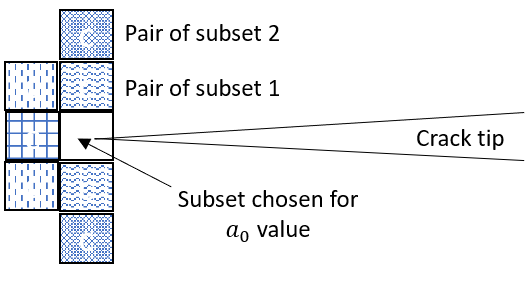
\includegraphics[scale=0.7]{Figures/Subset_choice}
%	\decoRule
%	\caption[Subset choice and pair of subset around]{Pair of subset around the $a_{0}$ subest chosen}
%	\label{fig:subest_chosen}
%\end{figure}
%
%To obtain CTOD, it is important to be careful to $a_{0}$ choice. Indeed, the chosen subset as presented on \ref{fig:subest_chosen}, will be determinant. Considering the image as a matrix composed of subset, the chosen subset as a position given by his m row and n column. To determinate the opening, it is necessary to have a look on the subsets in the same n column but at a different line. Indeed, the chosen subset will be the first one affected by the crack, that means, that information on the subset will not have importance anymore. While, looking to subset up and down allow to follow the displacement of the crack tip and measure it. The fact is to determine which pair of subsets is the best. The ones at the row n-1 and n+1, but maybe these ones will be on the crack at a given stage and will lose all the necessary information. That is why, an important choice must be done. Here COD pair was fixed equal to two. So the subset displacement analysed is the one of the pair of subset 2 on \ref{fig:subest_chosen}. Finally, by looking to these displacements, it is possible to obtain the value of the crack opening at each stages.
%
%%----------------------------------------------------------------------------------------
%%	SUBSECTION 4
%%----------------------------------------------------------------------------------------
%
%\subsection{Crack length analysis}
%
%At least, an important step in this code is the determination of $a_{DIC}$. This parameter is the crack length, which evolves with time during all the experiment. This factor is the most difficult to obtain, indeed tools as MatchID cannot help the user to obtain the result stage by stage. The value of a(t) will be equal to $a_{0}$ fixed by the user and additional to a $\Delta a$ which is the value of the crack length, evolving in time due to the applied force.
%
%\begin{customFrame}
%	roi = 'crop' # 'all'; 'crop'
%	i, incr = 1, 1
%	# incr : is used to step over stages if required (default = 1: all stages)
%	Y_i, Y_f = 0, UY.shape[0]
%	X_i, X_f = 0, a0.X
%\end{customFrame}
%
%\begin{customFrame}
%	# estimation of crack tip length
%	tipstep = np.zeros((alphaint.shape[0],1)) # unit: substep
%	tipmm = np.zeros((alphaint.shape[0],1)) # unit: mm
%	
%	for kk in np.arange(0,alphaint.shape[0],1):
%	alpha = alphaint[kk]
%	# Criterion for crack tip location
%	Kt = np.zeros(K.shape)
%	Kt[np.isnan(K)] = -1
%	Kt[K>=alpha*avgK] = 1
%	Ktemp = Kt
%	# n1 which must be relative to 'a0'
%	ind = np.argwhere(Ktemp==1)
%	row, col = ind[:,0], ind[:,1]
%	if len(col) == 0:
%	tipstep[kk] = 0
%	else:
%	tipstep[kk] = a0.X - np.min(col) # X component
%	# pixel>mm: [macro-pixel*(pixel/macro-pixel)*(mm/pixel)
%	tipmm[kk] = np.abs(tipstep[kk]*MatchID.mm2step - MatchID.mm2step)
%	
%	# for selected  alpha parameters you compute crack length
%	# crack length however should be ZERO at the beginning (no crack propagation)
%	ind = np.where(np.abs(tipmm - np.min(tipmm)) == 0)
%	alpha_alphasel = alphaint[ind[0][0]]
%\end{customFrame}
%A final part of the code allows to obtain a(t) depending on alpha  as it is done on \parencite{Reference14} article. It is done by a focus on the ZOI and the number of subsets composing it. Thanks to the matrix composed by every subsets, the displacement field can be observed. It is obtained by computing the distance between the center of a subset and it displacement from one image to the next one as shown in the literature review. To simplify the code, it is not done on every subset but only on the four corners. By computing the distance between the opposite corners, the maximum x-displacement and an y-displacement are input in a last matrix. 
%
%%----------------------------------------------------------------------------------------
%%	SUBSECTION 5
%%----------------------------------------------------------------------------------------
%
%\subsection{Compliance and Energy values}
%
%As said in alpha parameter section, The last step is to compute the Compliance and then the Energy release rate. Indeed, all the necessary parameters are present in the Python variables. So by computing the formula \ref{eq:Energy release rate equation} the different matrix composed of all the values depending on the stage are used to obtain first a compliance matrix with same dimensions of the CTOD and the dispacement of the Hydraulic press matrix created.
%
%\begin{customFrame}
%	ALP = (Test.load*Test.load)/(2*Test.thickness)
%	print(ALP)
%	
%	C = Test.disp/Test.load
%	
%	BET = C/crackL_J_mm[:,4]
%	
%	G = ALP * BET
%	
%	fig, ax = plt.subplots(figsize=(7,5), dpi=80)
%	plt.plot(crackL_J_mm[:,0], G, 'b-.', linewidth=2, label='R-Curve alpha 1')
%	plt.plot(crackL_J_mm[:,1], G, 'r--', linewidth=2, label='R-Curve alpha 2')
%	plt.plot(crackL_J_mm[:,2], G, 'g-', linewidth=2, label='R-Curve alpha 3')
%	plt.plot(crackL_J_mm[:,3], G, 'k:', linewidth=2, label='R-Curve alpha 4')
%	plt.plot(crackL_J_mm[:,4], G, 'c-.', linewidth=2, label='R-Curve alpha 5')
%	plt.plot(crackL_J_mm[:,5], G, 'm:', linewidth=2, label='R-Curve alpha 6')
%	plt.plot(crackL_J_mm[:,6], G, 'y--', linewidth=2, label='R-Curve alpha 7')
%	plt.xlabel('Crack length, a(t), mm')
%	plt.ylabel('$G_{Ic}, mm$')
%	
%\end{customFrame}
%
%As presented in this part of the code, after calculating G, some plots are created. But as explained in "alpha" and "a determination" sections, the crack length depends on alpha parameter. So some curves are ploted depending on "a" matrix changing according to the alpha.And the best R-curves must be determined for the best crack length. It is necessary to find the best alpha parameter to have these final values.
%
%Finaly, 